\chapter{Dimensionamento das Cargas} \label{secao:modelagem_cargas}

\section{Introdução}

Para que seja possível simular e validar o sistema é necessário saber qual o seu consumo, de forma que é possível saber se o sistema atende os requisitos. Além disso, o dimensionamento das cargas possibilita o projeto dos conversores que as alimentam. Este capítulo apresenta o dimensionamento das cargas de todo o sistema, incluindo o computador de bordo, os rádios, o sistema de energia e os \textit{payloads}.

\section{Computador de Bordo}

O computador de bordo tem funções como armazenamento dos dados em memória não-volátil, leitura de sensores e aquisição dos dados dos demais módulos do satélite.

Alguns contribuintes para o consumo estão listados na tabela \ref{consumo_computador_bordo}. Como é possível observar, poucos componentes contribuem para a maior parte do consumo. O cálculo da potência consumida é realizado multiplicando a corrente consumida pela tensão de alimentação, de \SI{3,3}{\volt}, exceto em casos especiais onde a equação é fornecida pelo \textit{datasheet} do componente.

\begin{table}[!htpb]
\centering
\begin{tabular}{c c c c}
\\ \hline
Componente & Quantia & Corrente [\SI{}{\milli\ampere}] & Potência [\SI{}{\milli\watt}] \\ \hline \hline
\glsentryshort{imu} (MPU-9250) & 1 & 3,7 \cite{mpu9250} & 12,21 \\
\glsentryshort{imu} (BMX055) & 1 & 5,7 \cite{bmx055} & 18,81 \\
Gerador de Referência & 1 & 0,026 \cite{ref5030}, \cite{msp430f6659} & 0,0008 \cite{ref5030} \\
Amplificador Operacional & 4 & 0,2 \cite{tlv341} & 2,64 \\
\textit{Watchdog} Externo & 1 & 0,025 \cite{tps3823} & 0,0825 \\
microSD & 1 & 0,25 \cite{microSD} & 0,825 \\
Memória não-volátil & 3 & 0,05 \cite{is25lp128} & 0,495 \\
Microcontrolador & 1 & 8,39 \cite{msp430f6659} & 57,1134 \cite{msp430f6659} \\
Sensor de Corrente & 1 & 0,23 \cite{max9934} & 2,277 \\
Resistor Shunt (\SI{0,05}{\ohm}) & 1 & 19,271 & 0,01857 \\ \hline
Total & - & 19,271 & 94,47 \\ \hline
\end{tabular}
\caption{Consumo do Computador de Bordo}
\label{consumo_computador_bordo}
\end{table}

Aqui foram considerados apenas os consumos constantes, ou seja, o aumento no consumo durante comunicações do processador com outros dispositivos não foi considerado por apresentar um valor muito pequeno quando comparado com o constante (\SI{0,05}{\milli\watt} de média).

\section{Rádios e Amplificadores de Potência}

Os dois rádios do satélite têm como função enviar os dados coletados para a terra, através de telemetria. Durante a transmissão o consumo de potência é muito maior do que em outros momentos, devido ao fato de que o \gls{pa} de cada rádio fica ativo somente durante transmissões. Portanto para modelar o consumo deste sistema será considerado apenas o comportamento dinâmico, de acordo com a tabela \ref{consumo_radios}. Cada rádio envia periodicamente dados para a Terra, com períodos de transmissão e o tempo ativo diferentes. Além disso, existe a possibilidade de a estação terrestre solicitar o envio de dados através de telecomandos. Neste caso, a transmissão fica ativa até que todos os dados solicitados sejam enviados. Para modelar este comportamento será considerada uma janela de 10 minutos por órbita, o que simula um hipotético pior caso (em termos de energia consumida). Cada /gls{pa} é alimentado com \SI{5}{\volt}.

\begin{table}[!htpb]
\centering
\begin{tabular}{c c c c}
\\ \hline
Componente & Período/ & Corrente [\SI{}{\ampere}] & Potência [\SI{}{watt}] \\
& Tempo Ativo [\SI{}{\second}] & & \\ \hline \hline
\glsentryshort{pa} (Transceiver) & 60/2 & 0,396 \cite{rf6886} & 1,98 \\
\glsentryshort{pa} (Beacon) & 10/0,6 & 0,396 \cite{rf6886} & 1,98 \\ \hline
Total & - & - & - \\ \hline
\end{tabular}
\caption{Consumo dos Rádios}
\label{consumo_radios}
\end{table}

\section{Sistema de Energia}

O \gls{eps} tem como função captar a energia dos painéis solares, armazenar em baterias e distribuir para os outros módulos. Estas funções geram o consumo detalhado na tabela \ref{consumo_eps}.

\begin{table}[!htpb]
\centering
\begin{tabular}{c c c c}
\\ \hline
Componente & Quantia & Corrente [\SI{}{\milli\ampere}] & Potência [\SI{}{\milli\watt}] \\ \hline \hline
Gerador de Referência & 1 & 0,026 \cite{ref5030}, \cite{msp430f6659} & 0,0008 \cite{ref5030} \\
Amplificador Operacional & 5 & 0,2 \cite{tlv341} & 0,66 \\
Sensor de Corrente & 7 & 0,23 \cite{max9934} & 0,759 \\
Resistor Shunt (\SI{0,75}{\ohm}) & 1 & 0,2 & 3 \\
Resistor Shunt (\SI{0,05}{\ohm}) & 6 & 508 & 12,903 \\
Timer 555 & 1 & 0,250 \cite{lmc555} & 0,825 \\
ADC externo & 1 & 0,59 \cite{ads1248} & 1,947 \\
Microcontrolador & 1 & 8,39 \cite{msp430f6659} & 57,1134 \cite{msp430f6659} \\
Kill-Switches & 4 & 350 & 3,063 \cite{si4403} \\
Monitor de Bateria & 1 & 0,135 \cite{ds2775} & 1,134 \cite{ds2775} \\
Proteção das Baterias & 1 & 700 & 10,29 \cite{fds6898az} \\
Aquecedor das Baterias & 2 & - & 3180\\
Conversor CC-CC (5420) & 1 & 49,456 & 206,588 \cite{tps5420} \\
Conversor CC-CC (5410) & 1 & 21,281 & 210,322 \cite{tps5410} \\
Conversor CC-CC (54540) & 2 & 600 & 149,032 \cite{tps54540} \\ \hline
Total & - & - & - \\ \hline
\end{tabular}
\caption{Consumo do Sistema de Energia}
\label{consumo_eps}
\end{table}

O Conversor CC-CC 5420 tem como função alimentar a parte digital dos rádios e o Sistema de Energia, portanto seu consumo é constante. Da mesma forma, o Conversor CC-CC 5410 tem como função alimentar o Computador de Bordo, portanto seu consumo também é constante. Por fim, o Conversor CC-CC 54540 tem como função alimentar o \gls{pa} de cada rádio, de forma que o seu consumo é dinâmico, com comportamento igual ao dos rádios. O aquecedor das baterias só é necessário nos momentos da órbita onde há eclipse (um terço da órbita), portanto assim será considerado para a modelagem.

Quando comparado com os outros módulos, este apresenta o maior consumo, porém isso acontece devido quase que somente aos aquecedores, que são componentes essenciais para o satélite.

\section{\textit{Payloads}}

Os \textit{Payloads} são os módulos do satélite que realizam o objetivo principal do satélite. Por exemplo, no caso de um satélite que tira fotos da terra os \textit{payloads} são as câmeras. No caso deste trabalho o \textit{payload} é um \gls{fpga} usado para testar os efeitos da radição nos componentes no espaço, com consumo de \SI{288}{\milli\ampere} em \SI{5}{\volt} (\SI{1,44}{\watt}), devido a presença do \gls{fpga} Xilinx Artix 7 XC7A200T.

\section{Conclusões}

Para melhor visualização das cargas do sistema, a curva de corrente de carga para três órbitas pode ser vista na figura \ref{figura_corrente_carga}. Estes valores de corrente correspondem a potência apresentada nas seções anteriores para um tensão de \SI{5}{\volt}, que é a tensão de saída do regulador utilizado na simulação.

O valor máximo de potência da carga é de \SI{5.785}{\watt}, quando há uma transmissão ocorrendo e os aquecedores estão ligados.

\begin{figure}[!htpb]
\begin{center}
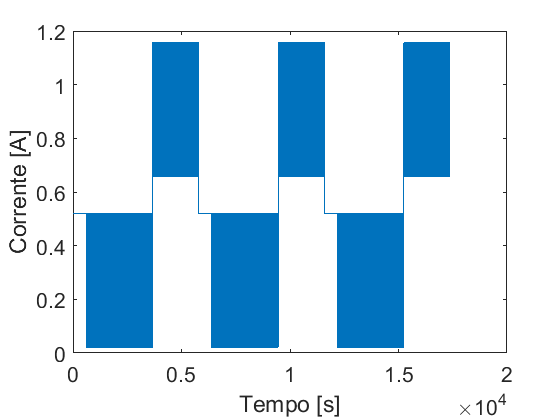
\includegraphics[scale=0.5]{figures/loadCurrent.png}
\end{center}
\caption{Corrente de Carga}
\label{figura_corrente_carga}
\end{figure}

Com isto é possível realizar a simulação do sistema.